\documentclass[11pt,a4paper]{scrartcl}

\usepackage[T1]{fontenc}
\usepackage[utf8]{inputenc}
\usepackage{kpfonts}
\usepackage[english]{babel}
\usepackage{amsmath,amssymb}
\usepackage[numbers,sort&compress]{natbib}
\usepackage[colorlinks=true,linkcolor=blue,citecolor=blue,urlcolor=blue]{hyperref}
\providecommand{\doi}[1]{\href{https://doi.org/#1}{doi: #1}}
\usepackage[margin=2.5cm]{geometry}
\usepackage{setspace}
\usepackage{enumitem}
\usepackage{graphicx}
\usepackage[automark,headsepline]{scrlayer-scrpage}
\usepackage{caption}

\onehalfspacing
\setkomafont{pagehead}{\small}

\graphicspath{{figures/}}

\lohead{\small HSAT2 hypothesis in PAIS --- Long Abstract}
\rohead{\small \pagemark}

\begin{document}
\emergencystretch 1em

\title{Could HSAT2 Repeat RNAs Drive Long COVID and ME/CFS?\\[4pt]
       A New Hypothesis}
\author{Olivier Croce\textsuperscript{1},
        Yannick Loth\textsuperscript{2},
        Patrick Lomonte\textsuperscript{3},\\[2pt]
        Alain Trautmann\textsuperscript{4},
        Genevi\`{e}ve Fourel\textsuperscript{1*}\\[4pt]
       \small
       \textsuperscript{1} LBMC, ENS Lyon, CNRS, Inserm, Lyon, France\\
       \textsuperscript{2} Independent researcher, Luxembourg\\
       \textsuperscript{3} Universit\'e Claude Bernard Lyon 1, France\\
       \textsuperscript{4} Independent researcher, France\\[0.5em]
       \small *Corresponding author: \texttt{genevieve.fourel@ens-lyon.fr}}
\date{July 2026 \\ \vspace{0.5em} \small Prepared for the ISLC-PAIS Conference 2026}
\maketitle

%%══════════════════════════════════════════════════════════════════
%% LONG ABSTRACT (verbatim per Geneviève Fourel)
%%══════════════════════════════════════════════════════════════════

Human satellite~2 (HSAT2) is a pericentromeric repeat representing
approximately 1.5\% of the human genome (Fig.~\ref{fig:genome}).
Under physiological conditions, it is transcriptionally silenced
through DNA methylation and packaging into a compact chromatin state
known as heterochromatin
\cite{Shadle2019HSATII,Gerard2023CTCFpreprint}.

\begin{figure}[htbp]
  \centering
  %% PLACEHOLDER -- AI-generated figure
  %% Genome organisation: centromere, pericentromere (HSAT2),
  %% telomere/subtelomere, transposable elements.  ~1.5% HSAT2,
  %% ~50% repetitive sequences, ~2% coding.
  
\includegraphics[width=0.85\textwidth]{fig1-genome-repeats}
  \caption{Organisation of the human genome.  Only $\sim$2\% encodes
           proteins; roughly half consists of repetitive sequences
           including centromeric, pericentromeric (home of HSAT2),
           telomeric/subtelomeric repeats, and transposable elements.
           In healthy cells these sequences are transcriptionally
           silenced by DNA methylation and compact
           heterochromatin (H3K9me3).}
  \label{fig:genome}
\end{figure}

In cancer, however, HSAT2 may become aberrantly expressed.  The
resulting HSAT2 RNAs can reprogram gene expression through molecular
mechanisms that are increasingly well understood
(Fig.~\ref{fig:mechanisms})
\cite{Ruzanov2024ETSsatelliteEV,Ninomiya2023CAST,Miyata2021CTCFsenescence}.
This reprogramming is not restricted
to the cells producing HSAT2 RNAs, as these RNAs are released into
body fluids within extracellular vesicles (EVs), allowing their
dissemination to distant tissues.

\begin{figure}[htbp]
  \centering
  %% PLACEHOLDER -- AI-generated figure
  %% Panel A: HSAT2 RNA as molecular sponge -- GGAA repeats
  %% sequester PU.1/ETS TFs and miRNAs.
  %% Panel B: CTCF sequestration alters 3D chromatin looping
  %% (normal vs disrupted side-by-side).
  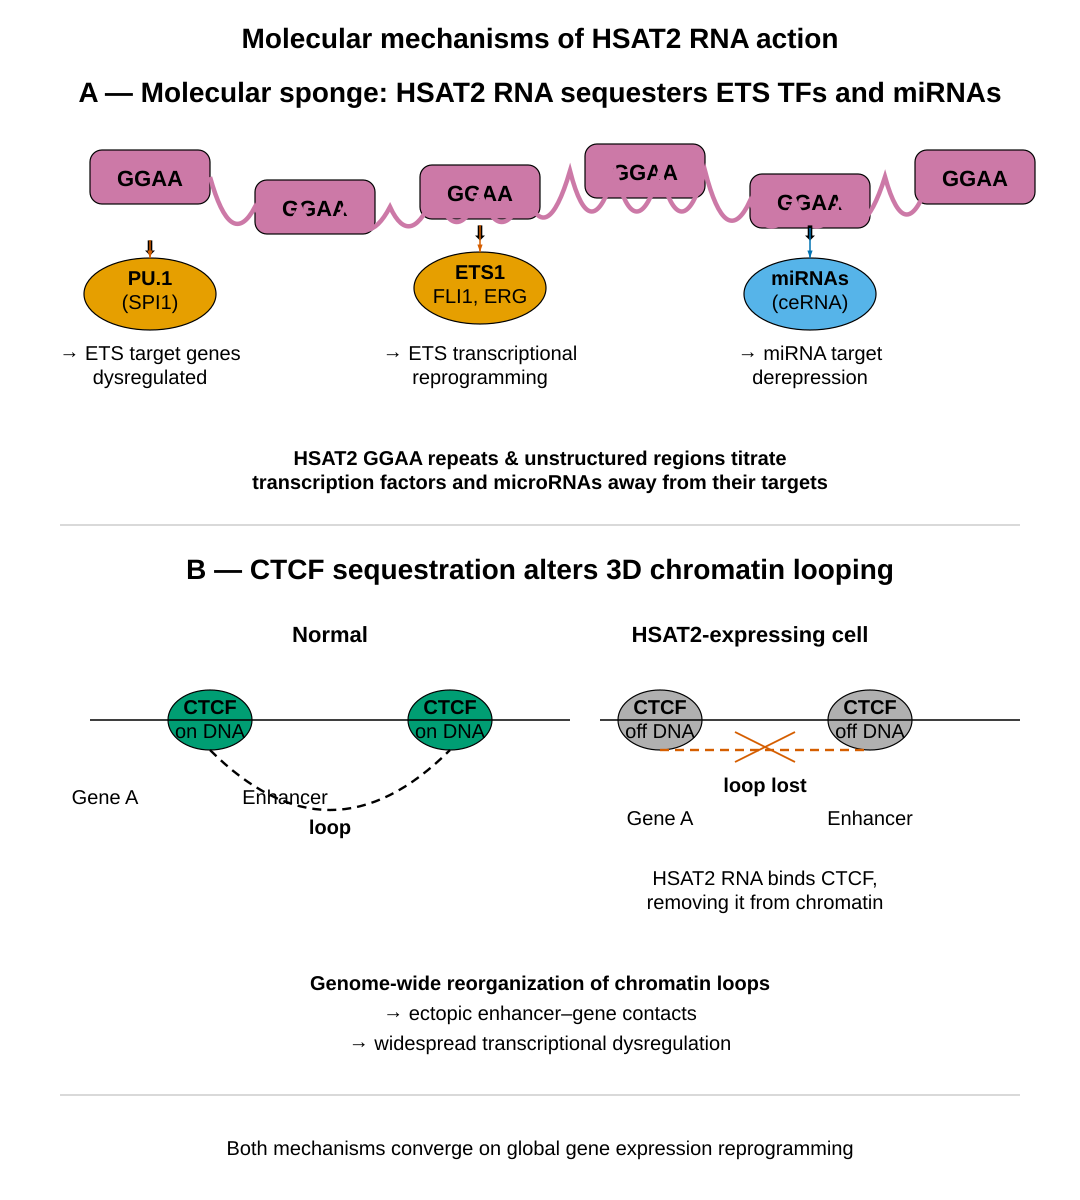
\includegraphics[width=0.90\textwidth]{fig2-molecular-mechanisms}
  \caption{Molecular mechanisms of HSAT2 RNA action.
           \textbf{(A)} Molecular sponge: HSAT2 RNA sequesters ETS
           family transcription factors (PU.1/SPI1 and others) via
           GGAA repeat motifs, and also acts as a ceRNA sponging
           miRNAs.  \textbf{(B)} CTCF sequestration alters
           genome-wide chromatin looping, producing widespread
           changes in gene expression.}
  \label{fig:mechanisms}
\end{figure}

In cancer, HSAT2 RNAs have been shown to impair several layers of
the body's defense mechanisms (Fig.~\ref{fig:immune}).  These
include innate immunity, which allows virtually every cell to defend
itself against viral infection, and the immune system, whose
specialized cells not only protect the body against pathogens but
also coordinate communication between organs and promote tissue
repair \cite{Ruzanov2024ETSsatelliteEV,Ninomiya2023CAST}.

\begin{figure}[htbp]
  \centering
  %% PLACEHOLDER -- AI-generated figure
  %% HSAT2 cell → EVs in bloodstream → uptake by immature myeloid
  %% cells → MDSC expansion → NK suppression + CD8 exhaustion
  %% (IL-10, IL-35, IDO1, TGF-β). Feed-forward loop back to EV
  %% production.
  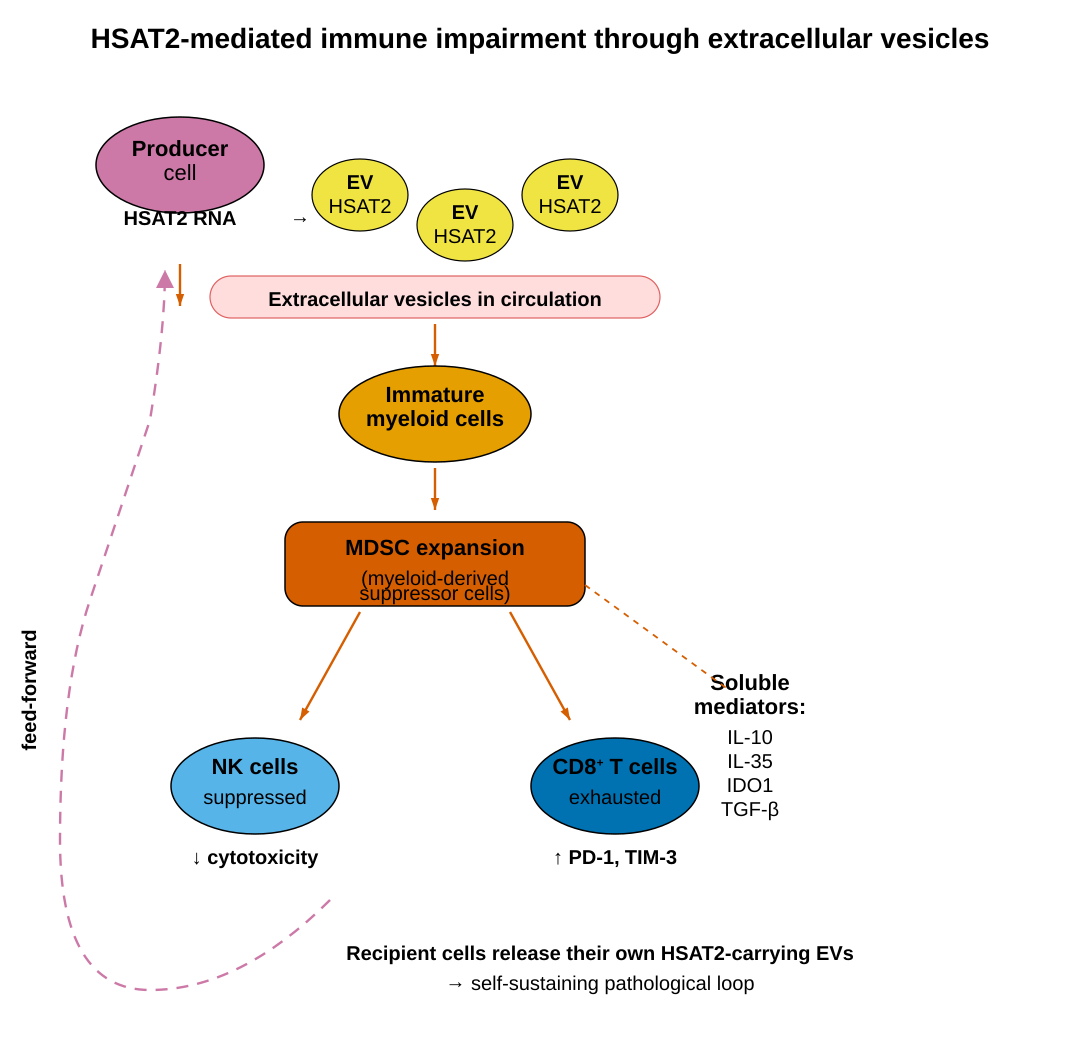
\includegraphics[width=0.90\textwidth]{fig3-immune-impairment}
  \caption{HSAT2-mediated immune impairment through extracellular
           vesicles.  HSAT2-laden EVs released from producing cells
           are taken up by immature myeloid cells, driving MDSC
           expansion.  MDSCs in turn suppress NK cells and drive
           CD8\textsuperscript{+} T-cell exhaustion via soluble
           mediators.  Recipient cells release their own
           HSAT2-carrying EVs, establishing a self-sustaining
           feed-forward loop.}
  \label{fig:immune}
\end{figure}

Here we propose that an analogous mechanism, involving HSAT2 RNAs as
a central player, may contribute to the development of post-acute
infection syndromes (PAIS), including Long COVID and ME/CFS.  Our
attention was drawn to this possibility by the observation that
HSAT2 RNAs are induced following herpesvirus infection or
reactivation \cite{Nogalski2019HSATII,Lahaye2025centromere}.
This may therefore provide a potential explanation
for the frequent observation that Long COVID and ME/CFS emerge
following reactivation of latent herpesviruses
\cite{Davis2021LongCOVIDreview,Komaroff2021PAISreview}.

Herpesvirus replication disrupts centromere organization and can
induce RNA synthesis from pericentromeric satellite repeats,
including HSAT2 (Fig.~\ref{fig:anatomy})
\cite{Lahaye2025centromere,Nogalski2019HSATII}.  Because each herpesvirus
preferentially infects only one or a limited number of cell types,
the critical initiation of HSAT2 RNA production may occur in
different cellular compartments depending on the virus involved.
For example, among herpesviruses reported to reactivate in Long
COVID, HSV-1 establishes latency primarily in sensory neurons, EBV
in memory B cells, HHV-6 in cells of the central nervous system and
the immune system, and HCMV in cells of the myeloid lineage,
endothelial cells lining blood vessels, and other tissue-resident
cells.

\begin{figure}[htbp]
  \centering
  %% PLACEHOLDER -- AI-generated figure
  %% Sagittal head/brain view: brainstem (inflamed, SARS-CoV-2),
  %% trigeminal ganglion (HSV-1 latency). Arrows showing proximity.
  %% Labels for EBV→B cells, HHV-6→CNS, HCMV→myeloid/endothelial.
  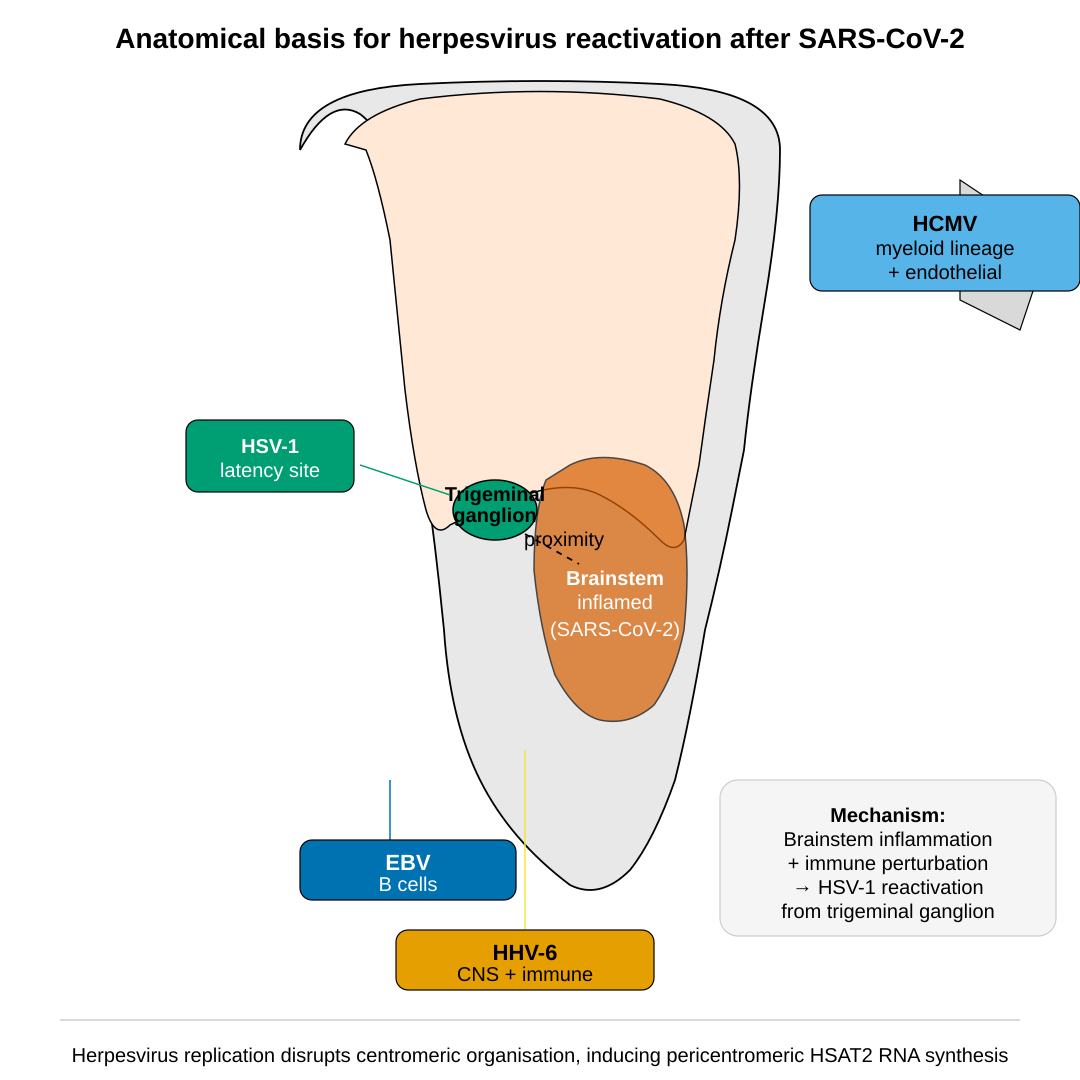
\includegraphics[width=0.80\textwidth]{fig4-anatomical-proximity}
  \caption{Anatomical basis for herpesvirus reactivation following
           SARS-CoV-2 infection.  HSV-1 establishes latency in the
           trigeminal ganglion, located in close anatomical proximity
           to the brainstem.  SARS-CoV-2-induced brainstem
           inflammation and immune perturbation may trigger HSV-1
           reactivation.  Other herpesviruses (HHV-6, EBV, HCMV)
           also establish latency in immune and central nervous
           system cells susceptible to COVID-19-mediated
           disruption.}
  \label{fig:anatomy}
\end{figure}

Following repeated or closely spaced viral infections, cumulative
changes in chromatin composition and DNA methylation of HSAT2
repeats may become sufficiently extensive to trigger significant
epigenetic erosion, ultimately establishing a permissive chromatin
state for HSAT2 repeat transcription
\cite{BonnetFourel2026ProAB,Shadle2019HSATII,Pappalardo2021repeats,
deVega2014methylation,Helliwell2020methylation,Peppercorn2025methylation}.  Once initiated, this state
could become self-sustaining through continued HSAT2 RNA production,
possibly in cooperation with additional mechanisms and eventually
involving multiple herpesviruses and multiple cell types.  Depending
on the magnitude of the initial epigenetic disruption, this
transition could also occur following a single episode of viral
reactivation.

By analogy with cancer, we hypothesize that vesicles released by
cells in which latent herpesviruses have reactivated and carrying
HSAT2 RNAs could spread from cell to cell, and potentially
throughout the body, in a manner similar to that of an infectious
agent, propagating this pathogenic signal and thereby driving
persistent immune dysregulation, particularly immune exhaustion
\cite{Ruzanov2024ETSsatelliteEV}.

Rather than presenting definitive proof, this short Perspective
assembles the available evidence into a coherent mechanistic
framework linking the initiating trigger to downstream molecular
events and clinical manifestations.  It also generates specific,
experimentally testable predictions that can now be investigated
using patient-derived samples
\cite{Seimiya2023HSATII,Yoruker2026HSAT2cfDNA,Seifert2026EVmiRNA,
Kishikawa2016SATII} (Fig.~\ref{fig:predictions}).

\begin{figure}[htbp]
  \centering
  %% PLACEHOLDER -- AI-generated figure
  %% Four panels: (1) blood→EV→HSAT2 measurement,
  %% (2) HSAT2+ vs HSAT2- subgroups, (3) combined biomarker panel,
  %% (4) methyl donors → EV HSAT2 reduction (with caution).
  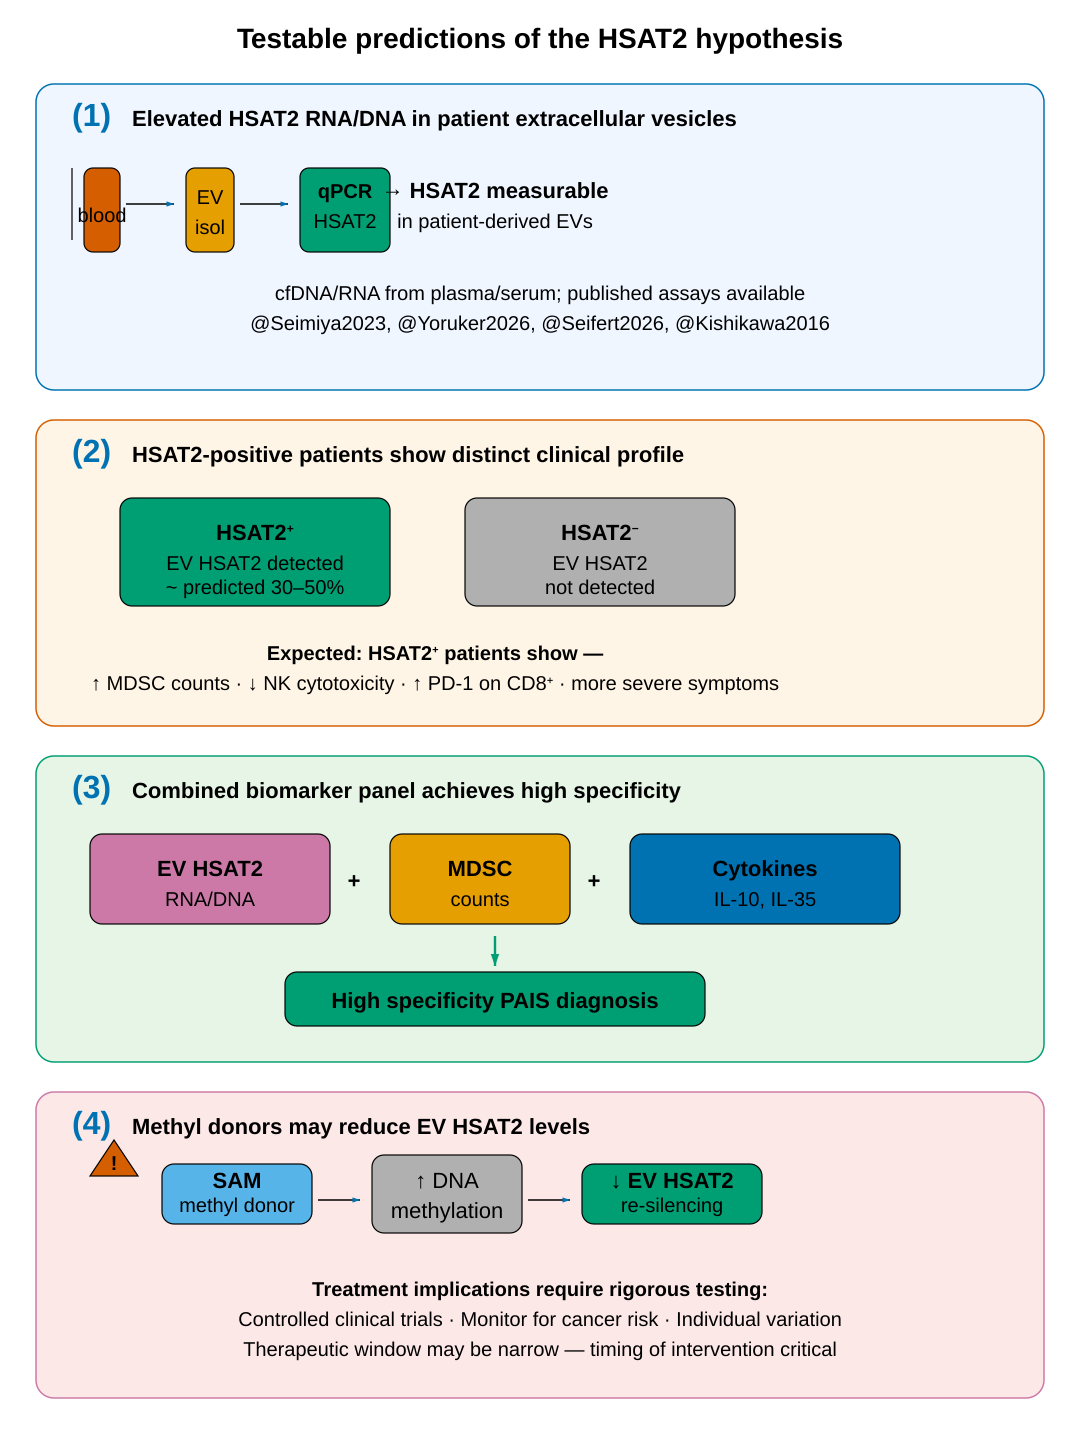
\includegraphics[width=0.90\textwidth]{fig5-predictions}
  \caption{Testable predictions of the HSAT2 hypothesis.
           (1)~Elevated HSAT2 RNA/DNA in patient EVs.
           (2)~HSAT2-positive patients show distinct clinical
           profile.  (3)~Combined biomarker panel achieves high
           specificity.  (4)~Methyl donors may reduce EV HSAT2.}
  \label{fig:predictions}
\end{figure}

Patients living with Long COVID and ME/CFS share a common goal:
recovery.  The fact that some patients recover without apparent
long-term sequelae strongly suggests that these disorders are, at
least in part, functional rather than irreversible, and are
maintained by self-reinforcing pathological feedback loops, possibly
involving multiple interacting mechanisms, rather than permanent
tissue destruction.  We propose that HSAT2 RNAs, both at their
initial sites of production and after dissemination throughout the
body via EVs, may represent one such mechanism, contributing to both
disease initiation and long-term maintenance.

At present, this remains a hypothesis.  However, if correct, it
would open an entirely new therapeutic perspective: neutralizing
extracellular HSAT2 RNAs could interrupt these pathological feedback
loops, allowing physiological regulatory networks to re-establish
themselves and thereby promoting recovery.

%%───── Bibliography ─────
\bibliographystyle{unsrtnat}
\bibliography{refs}

\end{document}
